\documentclass[14pt]{extbook}
\usepackage{multicol, enumerate, enumitem, hyperref, color, soul, setspace, parskip, fancyhdr} %General Packages
\usepackage{amssymb, amsthm, amsmath, bbm, latexsym, units, mathtools} %Math Packages
\everymath{\displaystyle} %All math in Display Style
% Packages with additional options
\usepackage[headsep=0.5cm,headheight=12pt, left=1 in,right= 1 in,top= 1 in,bottom= 1 in]{geometry}
\usepackage[usenames,dvipsnames]{xcolor}
\usepackage{dashrule}  % Package to use the command below to create lines between items
\newcommand{\litem}[1]{\item#1\hspace*{-1cm}\rule{\textwidth}{0.4pt}}
\pagestyle{fancy}
\lhead{Progress Quiz 2}
\chead{}
\rhead{Version B}
\lfoot{7862-5421}
\cfoot{}
\rfoot{Spring 2021}
\begin{document}

\begin{enumerate}
\litem{
Solve the quadratic equation below. Then, choose the intervals that the solutions $x_1$ and $x_2$ belong to, with $x_1 \leq x_2$.\[ 25x^{2} +60 x + 36 = 0 \]\begin{enumerate}[label=\Alph*.]
\item \( x_1 \in [-2.73, -2.18] \text{ and } x_2 \in [-0.7, -0.55] \)
\item \( x_1 \in [-2.18, 0.16] \text{ and } x_2 \in [-1.43, -1.16] \)
\item \( x_1 \in [-30.98, -28.84] \text{ and } x_2 \in [-30.05, -29.99] \)
\item \( x_1 \in [-4.74, -2.66] \text{ and } x_2 \in [-0.43, -0.35] \)
\item \( x_1 \in [-6.08, -4.26] \text{ and } x_2 \in [-0.26, -0.09] \)

\end{enumerate} }
\litem{
Solve the quadratic equation below. Then, choose the intervals that the solutions $x_1$ and $x_2$ belong to, with $x_1 \leq x_2$.\[ 25x^{2} +60 x + 36 = 0 \]\begin{enumerate}[label=\Alph*.]
\item \( x_1 \in [-4.46, -2.53] \text{ and } x_2 \in [-0.44, -0.3] \)
\item \( x_1 \in [-6.25, -5.12] \text{ and } x_2 \in [-0.29, -0.06] \)
\item \( x_1 \in [-30.46, -29.13] \text{ and } x_2 \in [-30.19, -29.83] \)
\item \( x_1 \in [-2.02, -1.16] \text{ and } x_2 \in [-1.22, -1.09] \)
\item \( x_1 \in [-3.48, -1.75] \text{ and } x_2 \in [-0.8, -0.45] \)

\end{enumerate} }
\litem{
Write the equation of the graph presented below in the form $f(x)=ax^2+bx+c$, assuming  $a=1$ or $a=-1$. Then, choose the intervals that $a, b,$ and $c$ belong to.
\begin{center}
    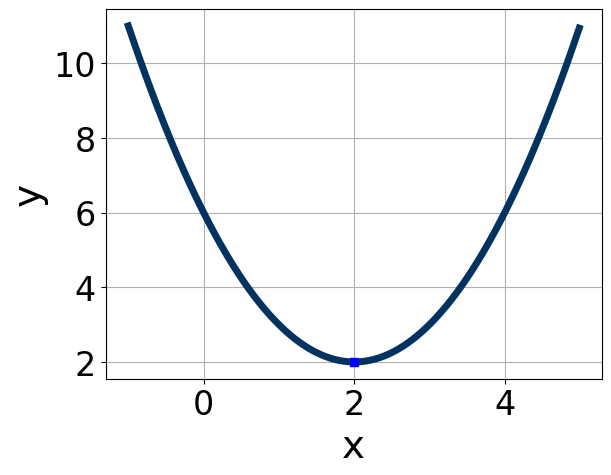
\includegraphics[width=0.5\textwidth]{../Figures/quadraticGraphToEquationCopyB.png}
\end{center}
\begin{enumerate}[label=\Alph*.]
\item \( a \in [-2, 0], \hspace*{5mm} b \in [6, 10], \text{ and } \hspace*{5mm} c \in [-24, -19] \)
\item \( a \in [0, 3], \hspace*{5mm} b \in [6, 10], \text{ and } \hspace*{5mm} c \in [19, 23] \)
\item \( a \in [-2, 0], \hspace*{5mm} b \in [6, 10], \text{ and } \hspace*{5mm} c \in [-12, -9] \)
\item \( a \in [0, 3], \hspace*{5mm} b \in [-9, -5], \text{ and } \hspace*{5mm} c \in [19, 23] \)
\item \( a \in [-2, 0], \hspace*{5mm} b \in [-9, -5], \text{ and } \hspace*{5mm} c \in [-12, -9] \)

\end{enumerate} }
\litem{
Solve the quadratic equation below. Then, choose the intervals that the solutions belong to, with $x_1 \leq x_2$ (if they exist).\[ -20x^{2} +8 x + 4 = 0 \]\begin{enumerate}[label=\Alph*.]
\item \( x_1 \in [-14.07, -13.78] \text{ and } x_2 \in [4.1, 6.2] \)
\item \( x_1 \in [-0.63, 0.1] \text{ and } x_2 \in [0.5, 2.2] \)
\item \( x_1 \in [-0.72, -0.52] \text{ and } x_2 \in [-0.6, 0.5] \)
\item \( x_1 \in [-19.75, -19.19] \text{ and } x_2 \in [18.1, 20.2] \)
\item \( \text{There are no Real solutions.} \)

\end{enumerate} }
\litem{
Write the equation of the graph presented below in the form $f(x)=ax^2+bx+c$, assuming  $a=1$ or $a=-1$. Then, choose the intervals that $a, b,$ and $c$ belong to.
\begin{center}
    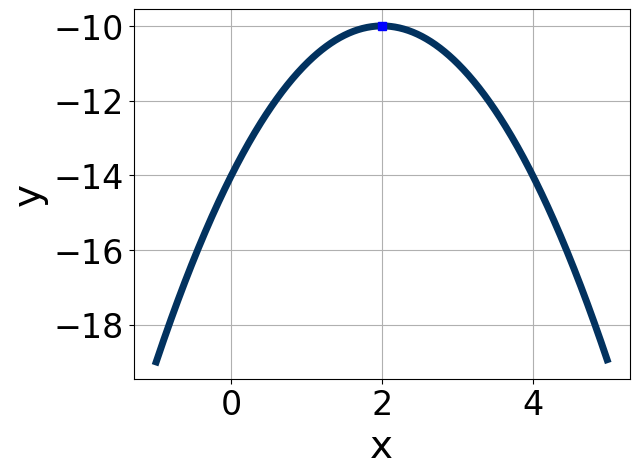
\includegraphics[width=0.5\textwidth]{../Figures/quadraticGraphToEquationB.png}
\end{center}
\begin{enumerate}[label=\Alph*.]
\item \( a \in [-2, 0], \hspace*{5mm} b \in [-6, -1], \text{ and } \hspace*{5mm} c \in [-10, -8] \)
\item \( a \in [-2, 0], \hspace*{5mm} b \in [3, 5], \text{ and } \hspace*{5mm} c \in [-10, -8] \)
\item \( a \in [1, 2], \hspace*{5mm} b \in [3, 5], \text{ and } \hspace*{5mm} c \in [-2, 0] \)
\item \( a \in [-2, 0], \hspace*{5mm} b \in [-6, -1], \text{ and } \hspace*{5mm} c \in [0, 4] \)
\item \( a \in [1, 2], \hspace*{5mm} b \in [-6, -1], \text{ and } \hspace*{5mm} c \in [-2, 0] \)

\end{enumerate} }
\litem{
Graph the equation below.\[ f(x) = -(x-2)^2 + 17 \]\begin{enumerate}[label=\Alph*.]
\begin{multicols}{2}\item 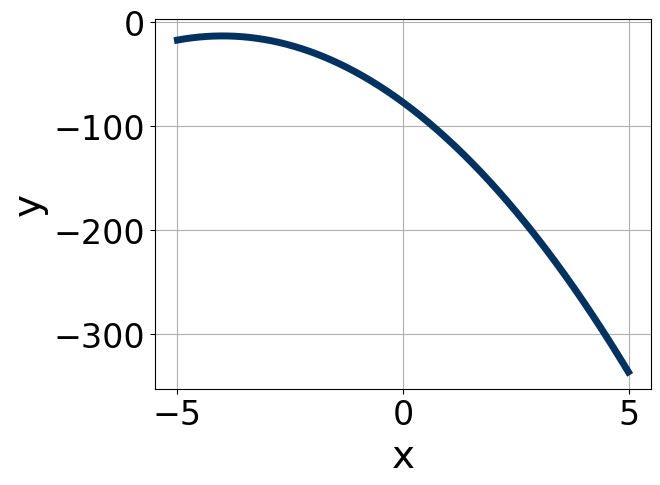
\includegraphics[width = 0.3\textwidth]{../Figures/quadraticEquationToGraphCopyAB.png}\item 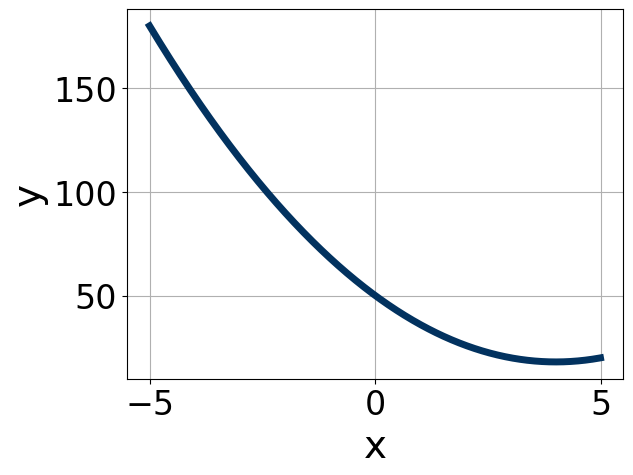
\includegraphics[width = 0.3\textwidth]{../Figures/quadraticEquationToGraphCopyBB.png}\item 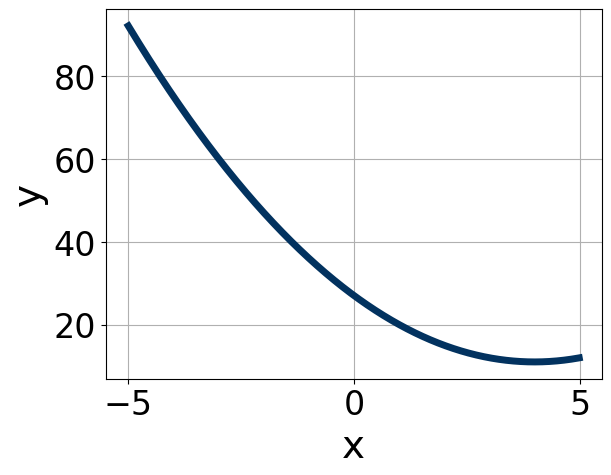
\includegraphics[width = 0.3\textwidth]{../Figures/quadraticEquationToGraphCopyCB.png}\item 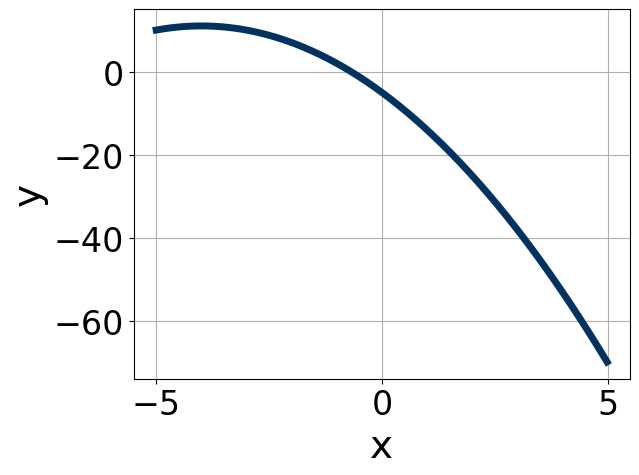
\includegraphics[width = 0.3\textwidth]{../Figures/quadraticEquationToGraphCopyDB.png}\end{multicols}\item None of the above.
\end{enumerate} }
\litem{
Graph the equation below.\[ f(x) = (x-3)^2 + 12 \]\begin{enumerate}[label=\Alph*.]
\begin{multicols}{2}\item 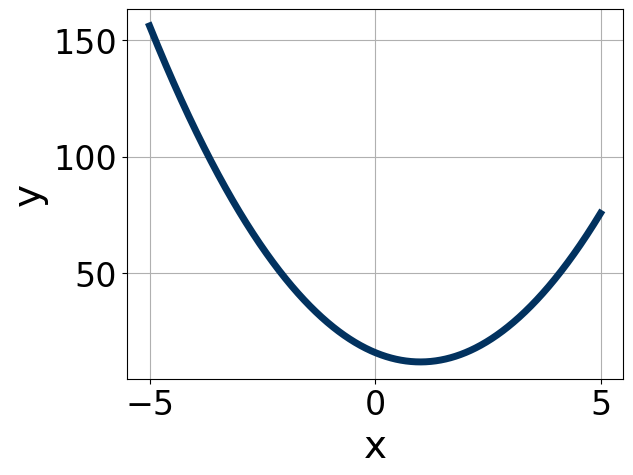
\includegraphics[width = 0.3\textwidth]{../Figures/quadraticEquationToGraphAB.png}\item 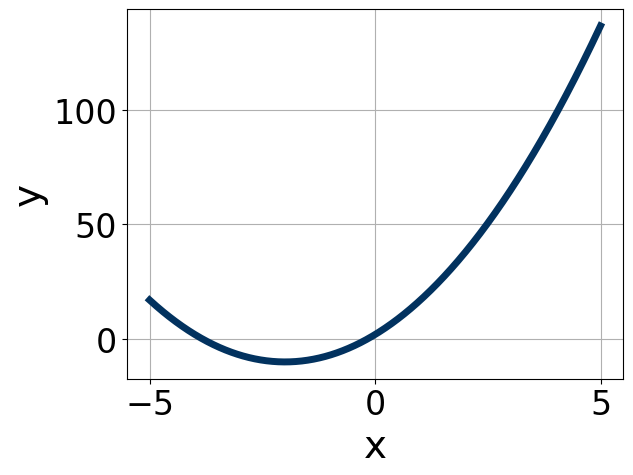
\includegraphics[width = 0.3\textwidth]{../Figures/quadraticEquationToGraphBB.png}\item 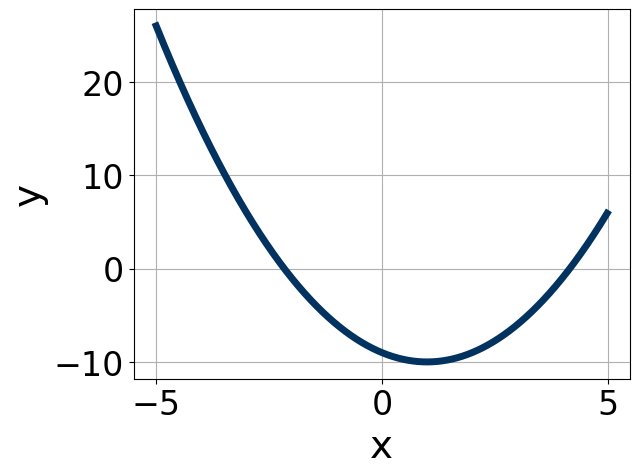
\includegraphics[width = 0.3\textwidth]{../Figures/quadraticEquationToGraphCB.png}\item 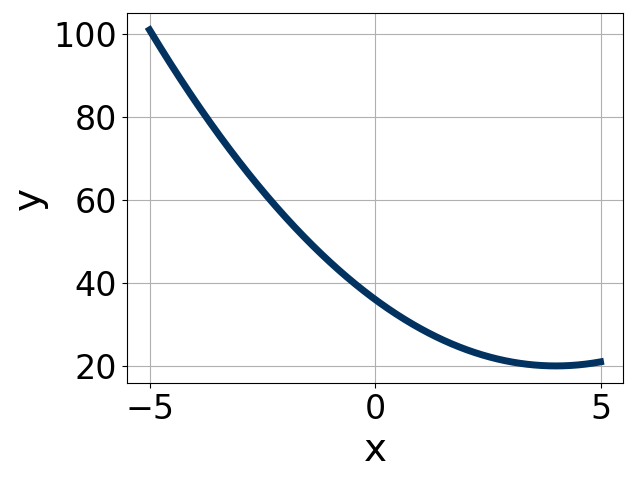
\includegraphics[width = 0.3\textwidth]{../Figures/quadraticEquationToGraphDB.png}\end{multicols}\item None of the above.
\end{enumerate} }
\litem{
Factor the quadratic below. Then, choose the intervals that contain the constants in the form $(ax+b)(cx+d); b \leq d.$\[ 36x^{2} +37 x -10 \]\begin{enumerate}[label=\Alph*.]
\item \( a \in [26.2, 27.6], \hspace*{5mm} b \in [-4, 1], \hspace*{5mm} c \in [0.5, 2.4], \text{ and } \hspace*{5mm} d \in [2, 9] \)
\item \( a \in [-1.9, 3.9], \hspace*{5mm} b \in [-8, -6], \hspace*{5mm} c \in [0.5, 2.4], \text{ and } \hspace*{5mm} d \in [44, 47] \)
\item \( a \in [3.7, 4.6], \hspace*{5mm} b \in [-4, 1], \hspace*{5mm} c \in [4.8, 10.4], \text{ and } \hspace*{5mm} d \in [2, 9] \)
\item \( a \in [8.1, 10.9], \hspace*{5mm} b \in [-4, 1], \hspace*{5mm} c \in [1.1, 4.2], \text{ and } \hspace*{5mm} d \in [2, 9] \)
\item \( \text{None of the above.} \)

\end{enumerate} }
\litem{
Solve the quadratic equation below. Then, choose the intervals that the solutions belong to, with $x_1 \leq x_2$ (if they exist).\[ 12x^{2} -11 x -8 = 0 \]\begin{enumerate}[label=\Alph*.]
\item \( x_1 \in [-1.05, 0.13] \text{ and } x_2 \in [0.9, 2.3] \)
\item \( x_1 \in [-1.54, -1.01] \text{ and } x_2 \in [-1.4, 1.2] \)
\item \( x_1 \in [-6.53, -4.98] \text{ and } x_2 \in [16.7, 18.2] \)
\item \( x_1 \in [-22.63, -21.73] \text{ and } x_2 \in [22.3, 24.9] \)
\item \( \text{There are no Real solutions.} \)

\end{enumerate} }
\litem{
Factor the quadratic below. Then, choose the intervals that contain the constants in the form $(ax+b)(cx+d); b \leq d.$\[ 36x^{2} -60 x + 25 \]\begin{enumerate}[label=\Alph*.]
\item \( a \in [1.69, 2.02], \hspace*{5mm} b \in [-6, -3], \hspace*{5mm} c \in [15, 25], \text{ and } \hspace*{5mm} d \in [-11, 1] \)
\item \( a \in [0.33, 1.33], \hspace*{5mm} b \in [-33, -26], \hspace*{5mm} c \in [0, 2], \text{ and } \hspace*{5mm} d \in [-34, -26] \)
\item \( a \in [11.57, 12.34], \hspace*{5mm} b \in [-6, -3], \hspace*{5mm} c \in [2, 4], \text{ and } \hspace*{5mm} d \in [-11, 1] \)
\item \( a \in [5.49, 6.23], \hspace*{5mm} b \in [-6, -3], \hspace*{5mm} c \in [6, 11], \text{ and } \hspace*{5mm} d \in [-11, 1] \)
\item \( \text{None of the above.} \)

\end{enumerate} }
\end{enumerate}

\end{document}